\documentclass[12pt,a4paper]{article}

\usepackage[utf8]{inputenc}
\usepackage[spanish]{babel}
\usepackage{graphicx}
\usepackage{geometry}
\geometry{a4paper, margin=2.5cm}
\usepackage{xcolor}
\usepackage{listings}
\usepackage{booktabs}
\usepackage{amsmath}
\usepackage{subcaption}
\usepackage{float}
\usepackage[colorlinks=true, linkcolor=blue, urlcolor=blue]{hyperref}

\definecolor{codegreen}{rgb}{0,0.6,0}
\definecolor{codegray}{rgb}{0.5,0.5,0.5}
\definecolor{codepurple}{rgb}{0.58,0,0.82}
\definecolor{backcolour}{rgb}{0.95,0.95,0.92}

\lstdefinestyle{mystyle}{
    backgroundcolor=\color{backcolour},   
    commentstyle=\color{codegreen},
    keywordstyle=\color{magenta},
    numberstyle=\tiny\color{codegray},
    stringstyle=\color{codepurple},
    basicstyle=\ttfamily\footnotesize,
    breakatwhitespace=false,         
    breaklines=true,                 
    captionpos=b,                    
    keepspaces=true,                 
    numbers=left,                    
    numbersep=5pt,                  
    showspaces=false,                
    showstringspaces=false,
    showtabs=false,                  
    tabsize=2,
    literate={á}{{'a}}1 {é}{{'e}}1 {í}{{'i}}1 {ó}{{'o}}1 {ú}{{'u}}1
             {Á}{{'A}}1 {É}{{'E}}1 {Í}{{'I}}1 {Ó}{{'O}}1 {Ú}{{'U}}1
             {ñ}{{\~n}}1 {Ñ}{{\~N}}1
}
\lstset{style=mystyle}

\title{\Huge\textbf{PROYECTO ESP32} \\ \Large Sensor de Distancia Ultrasónico con Pantalla OLED \\ \vspace{0.5cm} \normalsize \textit{Medición de distancia en centímetros con HC-SR04 y visualización en pantalla OLED SSD1306}}
\author{Msc. Néstor Fabio Montoya Palacios}
\date{2026 \\ \vspace{0.2cm} \small Plataforma: ESP32 Dev Module}

\begin{document}

\maketitle
\tableofcontents
\newpage

% ══════════════════════════════════════════════════════════════
\section{Introducción}
% ══════════════════════════════════════════════════════════════

Este documento describe el proyecto ``Sensor de Distancia Ultrasónico con Pantalla OLED'', en el cual se utiliza un microcontrolador \textbf{ESP32} junto con un sensor ultrasónico \textbf{HC-SR04} para medir la distancia a objetos cercanos. La distancia medida se muestra simultáneamente en dos interfaces: el \textbf{monitor serial} del computador (a través del puerto USB) y una \textbf{pantalla OLED SSD1306} de 128$\times$64 píxeles conectada mediante el protocolo de comunicación \textbf{I2C}.

El sensor HC-SR04 emite pulsos ultrasónicos a una frecuencia de 40\,kHz y mide el tiempo que tarda el eco en regresar tras rebotar en un objeto. A partir de este tiempo, el microcontrolador calcula la distancia utilizando la velocidad del sonido en el aire. Este principio físico, conocido como \textbf{eco-localización}, es el mismo que emplean los murciélagos y los sistemas de sonar marítimo.

% ══════════════════════════════════════════════════════════════
\section{Objetivo del Proyecto}
% ══════════════════════════════════════════════════════════════

Implementar un sistema de medición de distancia por ultrasonido que:
\begin{itemize}
    \item Utilice el sensor HC-SR04 para medir distancias en un rango de 2 a 400\,cm.
    \item Calcule la distancia en centímetros a partir del tiempo de vuelo de la onda ultrasónica.
    \item Muestre la distancia medida en el \textbf{monitor serial} del Arduino IDE a 115\,200 baudios.
    \item Visualice la distancia en tiempo real en una \textbf{pantalla OLED SSD1306} de 0,96 pulgadas.
    \item Actualice las lecturas cada 500\,ms para una visualización fluida.
\end{itemize}

% ══════════════════════════════════════════════════════════════
\section{Materiales Necesarios}
% ══════════════════════════════════════════════════════════════

\begin{table}[h!]
\centering
\begin{tabular}{cll}
\toprule
\textbf{Cant.} & \textbf{Componente} & \textbf{Especificación} \\
\midrule
1 & ESP32 Dev Module & Microcontrolador dual-core con Wi-Fi/Bluetooth \\
1 & Sensor HC-SR04 & Sensor ultrasónico de distancia (2--400\,cm) \\
1 & Pantalla OLED SSD1306 & Display 128$\times$64 px, I2C, 0,96'' \\
1 & Protoboard & Placa de pruebas de 830 puntos \\
  & Cables jumper & Macho-macho y macho-hembra \\
1 & Cable USB & Para programación y alimentación \\
\bottomrule
\end{tabular}
\caption{Lista de materiales del proyecto Sensor de Distancia con Pantalla OLED}
\end{table}

% ══════════════════════════════════════════════════════════════
\section{Esquema de Conexión}
% ══════════════════════════════════════════════════════════════

El circuito conecta el sensor HC-SR04 y la pantalla OLED SSD1306 al ESP32. El sensor utiliza dos pines digitales (GPIO2 para Trig y GPIO4 para Echo), mientras que la pantalla OLED se comunica por el bus I2C estándar del ESP32 (GPIO21 para SDA y GPIO22 para SCL). Ambos dispositivos se alimentan con 3,3\,V del ESP32 (el HC-SR04 también puede funcionar con 5\,V).

\begin{figure}[H]
\centering
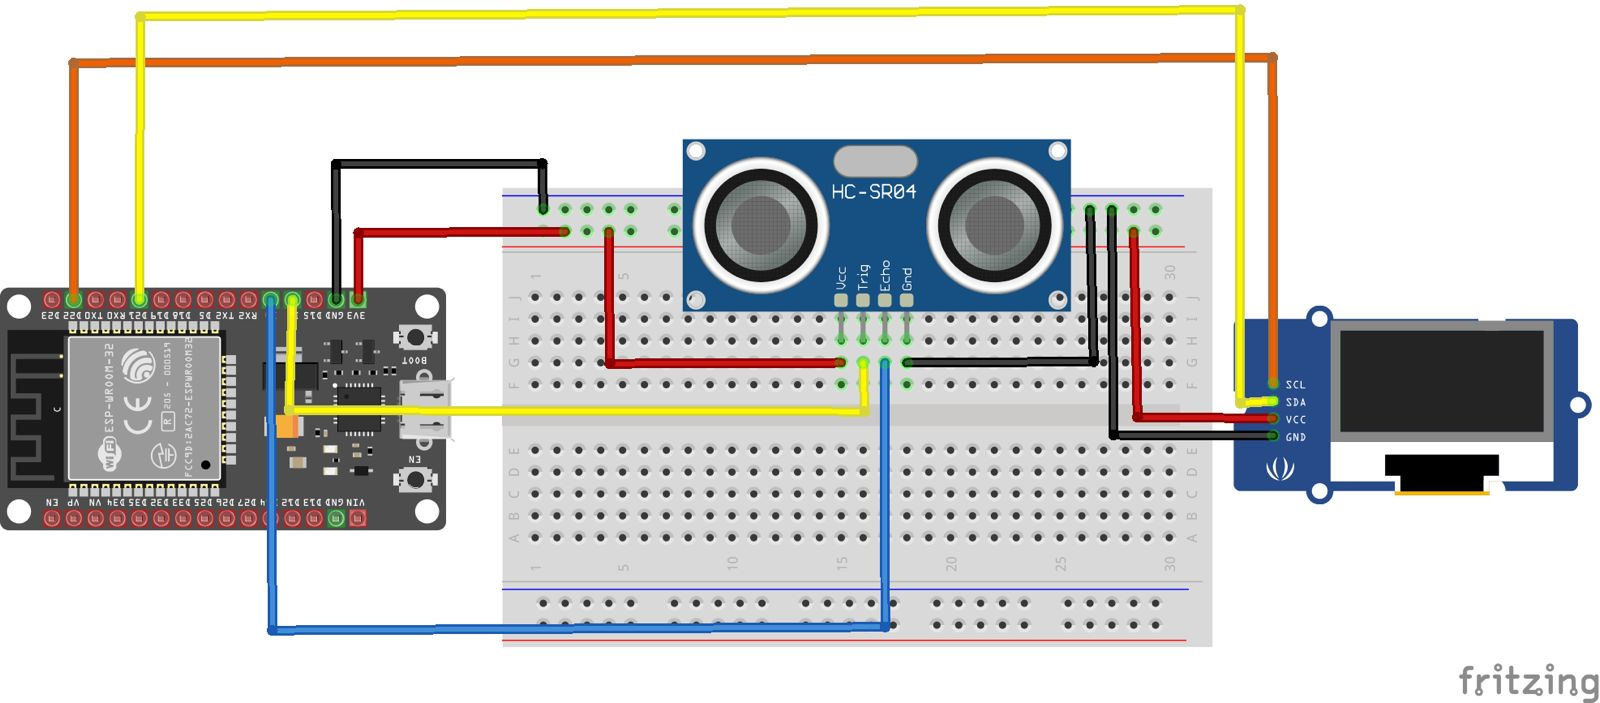
\includegraphics[width=0.85\textwidth]{../Esquemas/Sensor_de_distancia_con_pantalla_esq.jpeg}
\caption{Esquema de conexión del circuito en Fritzing -- ESP32 con HC-SR04 y pantalla OLED}
\label{fig:esquema}
\end{figure}

\subsection{Diagrama de Conexiones}

\begin{center}
\begin{tabular}{lll}
\toprule
\textbf{Componente} & \textbf{Pin} & \textbf{ESP32 GPIO} \\
\midrule
HC-SR04 & VCC & 3.3V (o 5V) \\
HC-SR04 & Trig & GPIO2 \\
HC-SR04 & Echo & GPIO4 \\
HC-SR04 & GND & GND \\
\midrule
OLED SSD1306 & VCC & 3.3V \\
OLED SSD1306 & GND & GND \\
OLED SSD1306 & SDA & GPIO21 (I2C SDA) \\
OLED SSD1306 & SCL & GPIO22 (I2C SCL) \\
\bottomrule
\end{tabular}
\end{center}

\textbf{Nota:} La pantalla OLED utiliza la dirección I2C \texttt{0x3C}, que es la dirección predeterminada de la mayoría de módulos SSD1306 de 128$\times$64 píxeles.

% ══════════════════════════════════════════════════════════════
\section{Código Fuente}
% ══════════════════════════════════════════════════════════════

A continuación se presenta el código completo del proyecto, que combina la lectura del sensor ultrasónico con la visualización en pantalla OLED mediante las librerías de Adafruit.

\subsection{Código Completo}
\lstinputlisting[language=C++, title=Sensor\_de\_distacia\_con\_pantalla.ino]{../Arduino/Sensor_de_distacia_con_pantalla/Sensor_de_distacia_con_pantalla.ino}

% ══════════════════════════════════════════════════════════════
\subsection{Análisis del Código}
% ══════════════════════════════════════════════════════════════

El código se organiza en tres secciones principales: inclusión de librerías y definición de constantes, función \texttt{setup()} para inicialización, y función \texttt{loop()} para el ciclo de medición continuo.

\subsubsection*{Librerías Utilizadas}

\begin{itemize}
    \item \textbf{\texttt{Wire.h}:} Librería estándar de Arduino que implementa el protocolo de comunicación I2C (Inter-Integrated Circuit). Es necesaria para la comunicación entre el ESP32 y la pantalla OLED a través de los pines SDA y SCL.
    \item \textbf{\texttt{Adafruit\_GFX.h}:} Librería gráfica base de Adafruit que proporciona primitivas de dibujo (texto, líneas, rectángulos, círculos). Sirve como capa de abstracción gráfica para múltiples tipos de displays.
    \item \textbf{\texttt{Adafruit\_SSD1306.h}:} Driver específico para pantallas OLED basadas en el controlador SSD1306. Extiende \texttt{Adafruit\_GFX} con funciones de inicialización y control propias de este chip.
\end{itemize}

\textbf{Instalación:} Ambas librerías de Adafruit se instalan desde el Gestor de Bibliotecas del Arduino IDE: \texttt{Programa $\rightarrow$ Incluir librería $\rightarrow$ Administrar bibliotecas $\rightarrow$} buscar ``Adafruit SSD1306'' e ``Adafruit GFX'' $\rightarrow$ instalar ambas.

\subsubsection*{Configuración de Pines y Display}

\begin{itemize}
    \item \textbf{trigPin = 2:} Pin de disparo del sensor HC-SR04 (salida digital).
    \item \textbf{echoPin = 4:} Pin de eco del sensor HC-SR04 (entrada digital).
    \item \textbf{SCREEN\_WIDTH = 128, SCREEN\_HEIGHT = 64:} Resolución de la pantalla OLED en píxeles.
    \item \textbf{OLED\_RESET = $-$1:} Se usa $-$1 porque el módulo OLED no tiene pin de reset dedicado (comparte el reset del ESP32).
\end{itemize}

\subsubsection*{Función \texttt{setup()}}

\begin{enumerate}
    \item Inicia la comunicación serial a 115\,200 baudios para depuración en el monitor serial.
    \item Inicializa la pantalla OLED con \texttt{display.begin(SSD1306\_SWITCHCAPVCC, 0x3C)}, donde \texttt{SSD1306\_SWITCHCAPVCC} indica que el display genera internamente el voltaje de 3,3\,V necesario, y \texttt{0x3C} es la dirección I2C del módulo.
    \item Limpia el búfer de la pantalla con \texttt{display.clearDisplay()}.
    \item Configura GPIO2 como salida (trigPin) y GPIO4 como entrada (echoPin).
\end{enumerate}

\subsubsection*{Función \texttt{loop()}}

El bucle principal ejecuta el ciclo completo de medición y visualización cada 500\,ms:

\begin{enumerate}
    \item \textbf{Generación del pulso ultrasónico:}
    \begin{itemize}
        \item Se pone el pin Trig en LOW durante 2\,$\mu$s para asegurar un estado limpio.
        \item Se genera un pulso HIGH de 10\,$\mu$s en el pin Trig, que ordena al HC-SR04 emitir una ráfaga de 8 pulsos ultrasónicos a 40\,kHz.
        \item Se regresa el pin Trig a LOW.
    \end{itemize}
    
    \item \textbf{Lectura del eco:} La función \texttt{pulseIn(echoPin, HIGH)} mide la duración en microsegundos del pulso HIGH en el pin Echo, que corresponde al tiempo de ida y vuelta de la onda ultrasónica.
    
    \item \textbf{Cálculo de la distancia:} Se aplica la fórmula:
    \begin{equation}
    d = \frac{t}{58{,}4}
    \label{eq:distancia}
    \end{equation}
    donde $d$ es la distancia en centímetros y $t$ es la duración del pulso en microsegundos.
    
    \item \textbf{Visualización serial:} Imprime ``Distancia: X.XX cm'' en el monitor serial.
    
    \item \textbf{Visualización OLED:} Limpia la pantalla, configura tamaño de texto 2 (16px de alto), escribe ``Distancia:'' en la parte superior y el valor numérico con unidades ``cm'' debajo, luego actualiza la pantalla con \texttt{display.display()}.
    
    \item \textbf{Pausa:} Espera 500\,ms antes de la siguiente medición.
\end{enumerate}

% ══════════════════════════════════════════════════════════════
\section{Principio de Funcionamiento}
% ══════════════════════════════════════════════════════════════

\subsection{El Sensor Ultrasónico HC-SR04}

El HC-SR04 es un sensor de distancia que utiliza ondas ultrasónicas (sonido a frecuencias superiores a los 20\,kHz, inaudibles para el oído humano) para medir la distancia a un objeto. Sus especificaciones principales son:

\begin{center}
\begin{tabular}{ll}
\toprule
\textbf{Parámetro} & \textbf{Valor} \\
\midrule
Voltaje de operación & 5\,V DC \\
Corriente de reposo & $<$ 2\,mA \\
Frecuencia de trabajo & 40\,kHz \\
Rango de medición & 2 -- 400\,cm \\
Ángulo efectivo & $<$ 15° \\
Resolución & 0,3\,cm \\
Señal de disparo & Pulso TTL de 10\,$\mu$s \\
\bottomrule
\end{tabular}
\end{center}

\subsection{Principio Físico: Eco-localización}

El funcionamiento se basa en la medición del \textbf{tiempo de vuelo} (\textit{Time of Flight}, ToF) de un pulso ultrasónico:

\begin{enumerate}
    \item El transductor emisor genera una ráfaga de 8 pulsos ultrasónicos a 40\,kHz.
    \item Las ondas viajan por el aire hasta impactar un objeto.
    \item El objeto refleja las ondas (eco) de vuelta hacia el sensor.
    \item El transductor receptor detecta el eco y genera un pulso eléctrico cuya duración es proporcional al tiempo de vuelo.
\end{enumerate}

La distancia se calcula con la ecuación fundamental:
\begin{equation}
d = \frac{v_s \times t}{2}
\label{eq:fisica}
\end{equation}

donde $v_s$ es la velocidad del sonido en el aire ($\approx 343$\,m/s a 20\,°C) y $t$ es el tiempo total de ida y vuelta. Se divide por 2 porque el sonido recorre el doble de la distancia (ida y vuelta).

Sustituyendo $v_s = 343$\,m/s $= 0{,}0343$\,cm/$\mu$s:
\begin{equation}
d\,[\text{cm}] = \frac{0{,}0343 \times t\,[\mu\text{s}]}{2} = \frac{t}{58{,}31} \approx \frac{t}{58{,}4}
\end{equation}

que es precisamente la fórmula utilizada en el código: \texttt{distance = duration / 58.4}.

\subsection{La Pantalla OLED SSD1306}

La pantalla OLED (Organic Light-Emitting Diode) SSD1306 es un display monocromático de 128$\times$64 píxeles que se comunica mediante I2C. A diferencia de las pantallas LCD retroiluminadas, cada píxel OLED emite su propia luz, lo que proporciona:

\begin{itemize}
    \item \textbf{Contraste infinito:} Los píxeles apagados son verdaderamente negros.
    \item \textbf{Bajo consumo:} Solo consume energía en los píxeles encendidos.
    \item \textbf{Ángulo de visión amplio:} Legible desde prácticamente cualquier ángulo.
    \item \textbf{Tamaño compacto:} El módulo de 0,96'' es ideal para proyectos embebidos.
\end{itemize}

\subsection{Protocolo I2C}

El bus I2C (\textit{Inter-Integrated Circuit}) utiliza solo dos líneas para la comunicación:
\begin{itemize}
    \item \textbf{SDA} (Serial Data): Línea de datos bidireccional (GPIO21 en ESP32).
    \item \textbf{SCL} (Serial Clock): Señal de reloj generada por el maestro (GPIO22 en ESP32).
\end{itemize}

El ESP32 actúa como \textit{maestro} y la pantalla OLED como \textit{esclavo} con dirección \texttt{0x3C}. Cada trama I2C incluye la dirección del esclavo, un bit de lectura/escritura y los datos a transmitir.

\subsection{Arquitectura del Sistema}

\begin{verbatim}
    Objeto           HC-SR04              ESP32              OLED SSD1306
    (obstáculo)  <-- Ultrasonido -->  GPIO2 (Trig)      GPIO21 (SDA) -->  Display
                     40 kHz          GPIO4 (Echo)      GPIO22 (SCL) -->  128x64
                     Eco                  |
                                          |
                                    Serial 115200
                                          |
                                          v
                                    Monitor Serial
                                    (Arduino IDE)
\end{verbatim}

% ══════════════════════════════════════════════════════════════
\section{Fotografías del Montaje}
% ══════════════════════════════════════════════════════════════

Las siguientes imágenes documentan el montaje físico del proyecto en funcionamiento.

\begin{figure}[H]
\centering
\begin{subfigure}[b]{0.48\textwidth}
    \centering
    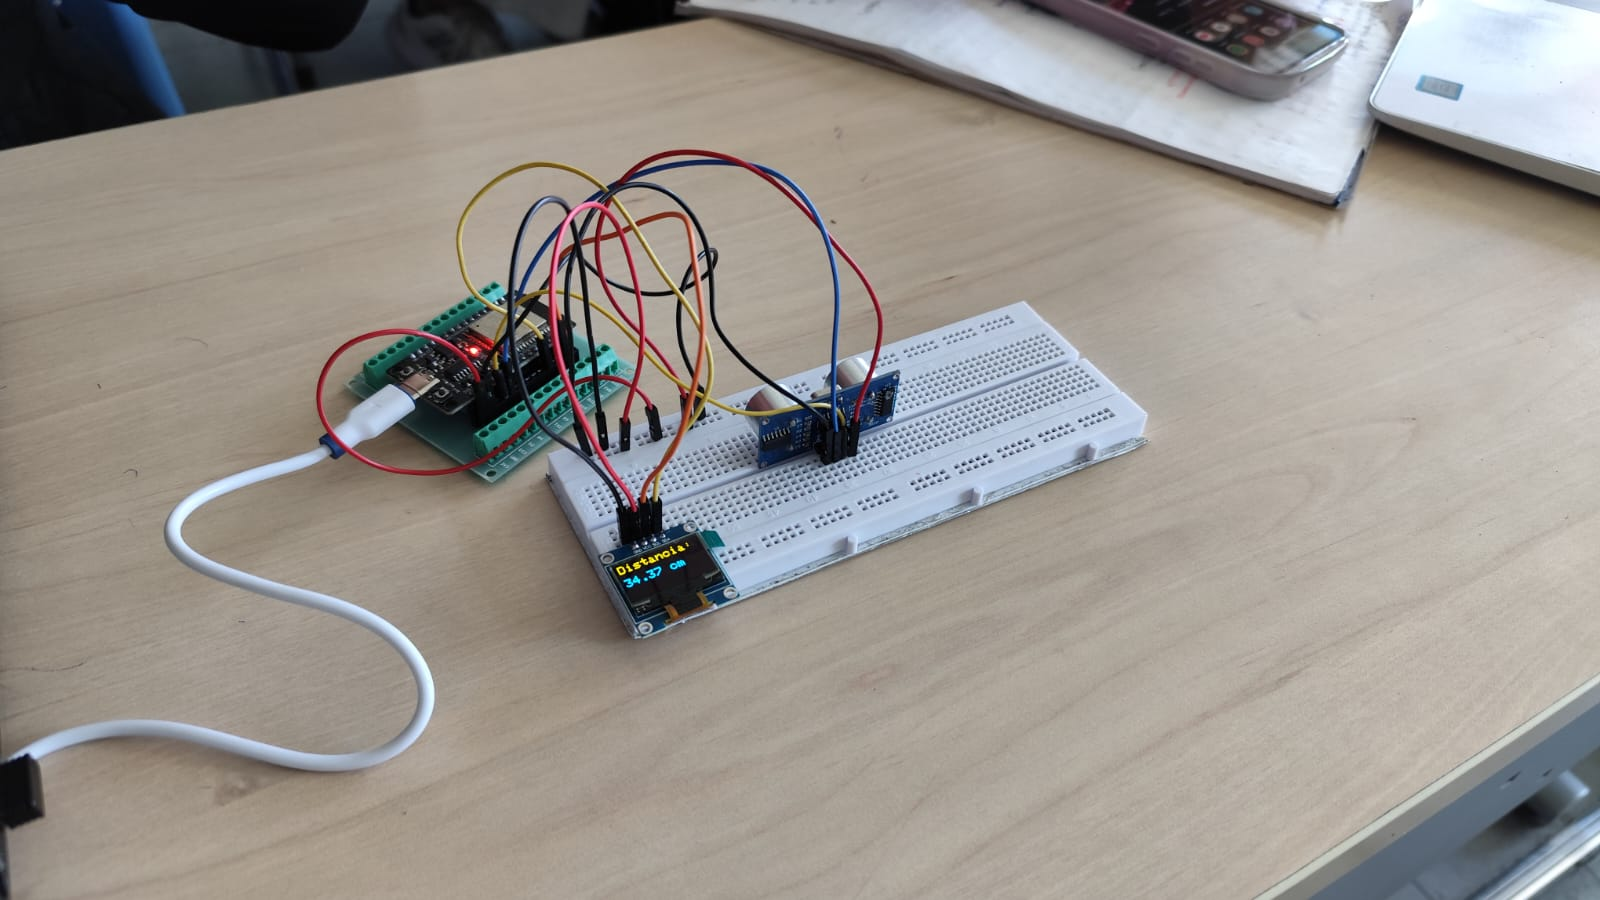
\includegraphics[width=\textwidth]{../Imagenes/Sensor_de_distacia_con_pantalla_imgs/Sensor_de_distancia_con_pantalla_img1.jpeg}
    \caption{Vista general del montaje: ESP32 en su base con bornera, conectado a la protoboard con el sensor HC-SR04 y la pantalla OLED mostrando la lectura de distancia en centímetros. Se observa el cable USB para alimentación y comunicación serial.}
    \label{fig:img1}
\end{subfigure}
\hfill
\begin{subfigure}[b]{0.48\textwidth}
    \centering
    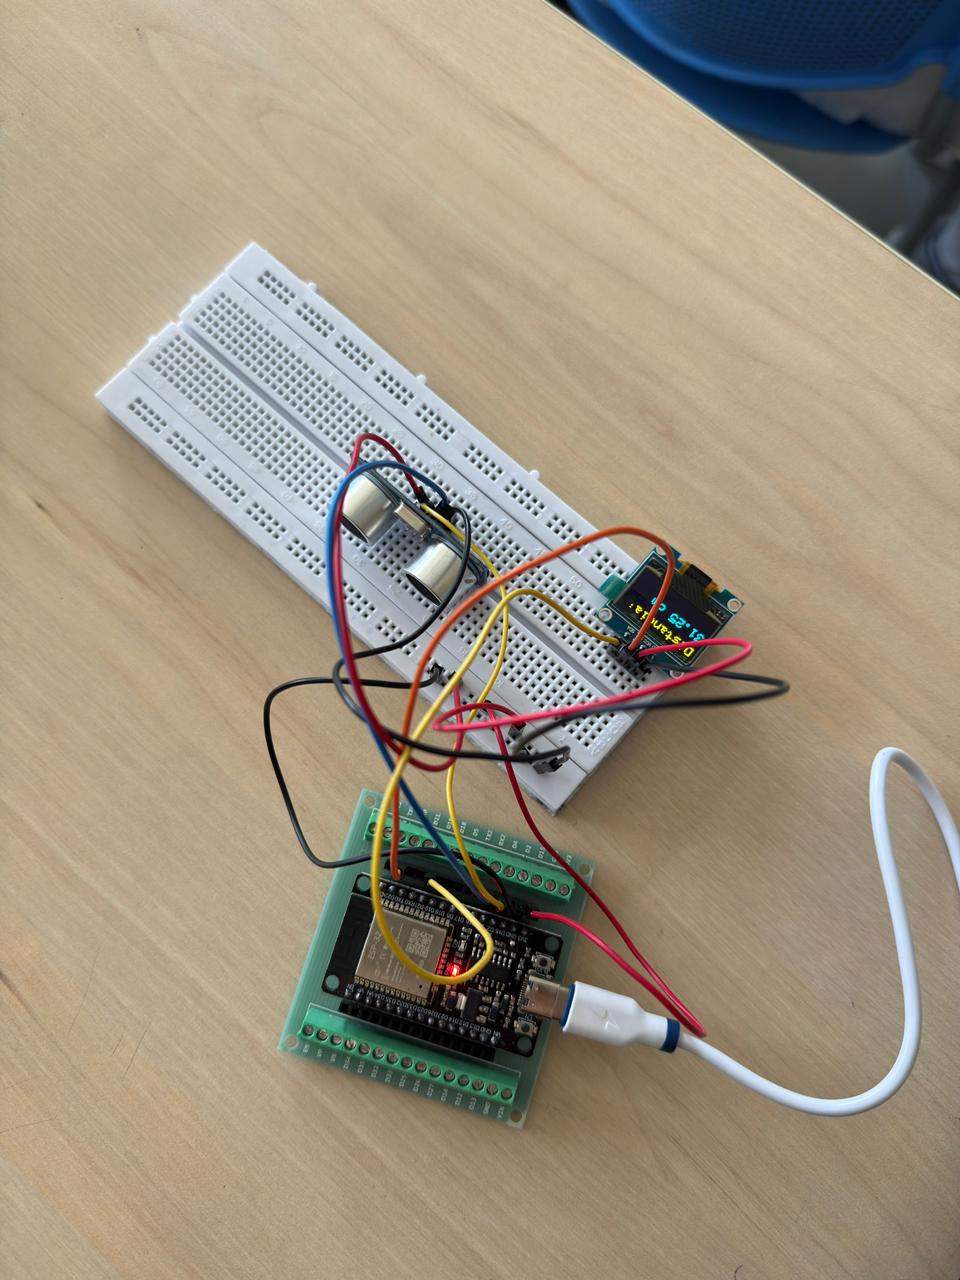
\includegraphics[width=\textwidth]{../Imagenes/Sensor_de_distacia_con_pantalla_imgs/Sensor_de_distancia_con_pantalla_img2.jpeg}
    \caption{Vista desde otro ángulo del circuito: se aprecia el sensor ultrasónico HC-SR04 montado en la protoboard, la pantalla OLED mostrando la distancia medida, y el ESP32 en su módulo de desarrollo con bornera verde.}
    \label{fig:img2}
\end{subfigure}
\caption{Montaje físico del sensor de distancia con pantalla OLED -- Vistas generales}
\label{fig:montaje1}
\end{figure}

\begin{figure}[H]
\centering
\begin{subfigure}[b]{0.48\textwidth}
    \centering
    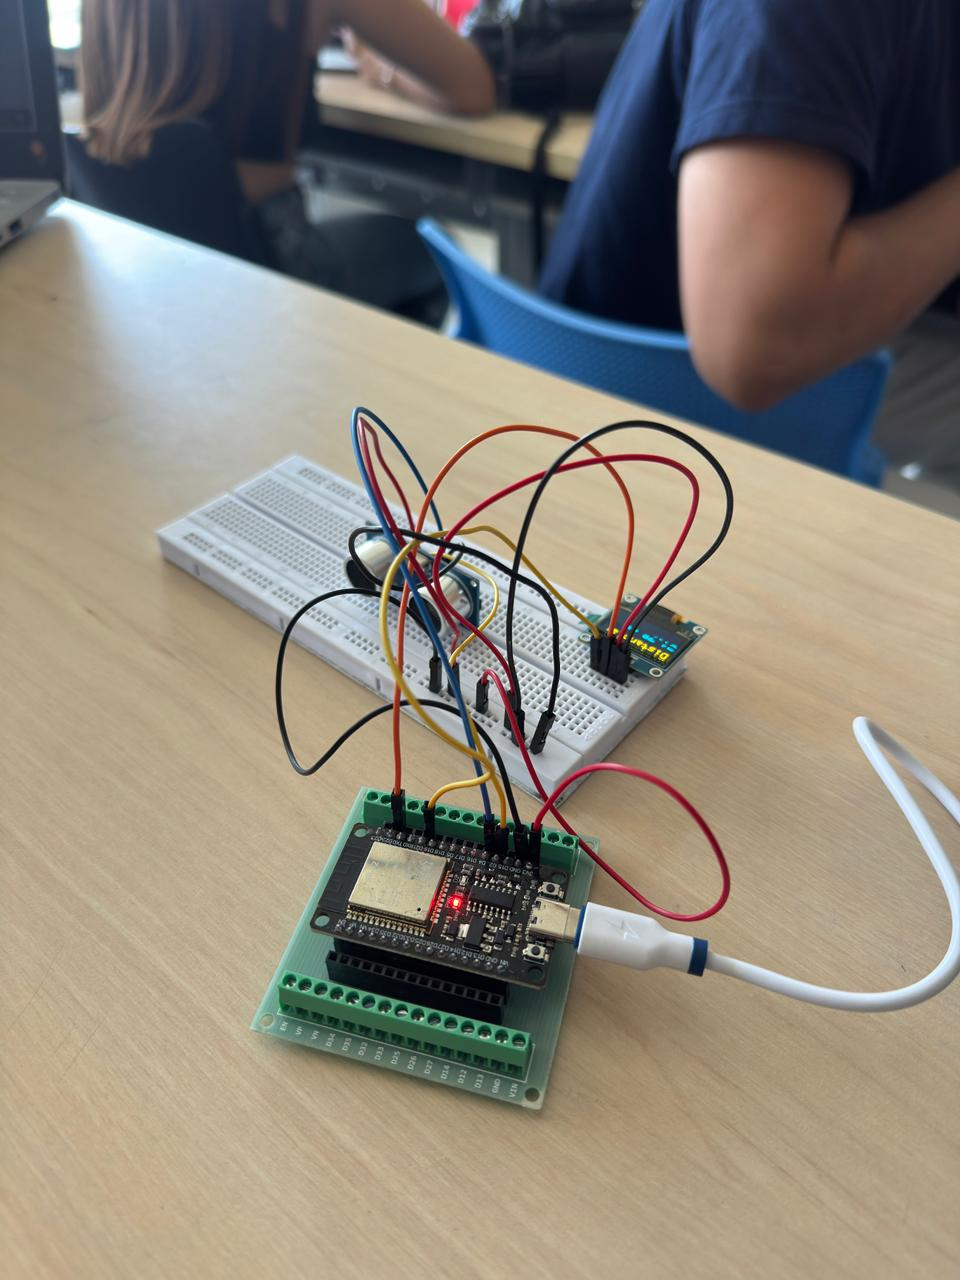
\includegraphics[width=\textwidth]{../Imagenes/Sensor_de_distacia_con_pantalla_imgs/Sensor_de_distancia_con_pantalla_img3.jpeg}
    \caption{Detalle del ESP32 en primer plano con su LED de estado encendido, mostrando las conexiones de cables hacia la protoboard donde se encuentran el sensor HC-SR04 y la pantalla OLED.}
    \label{fig:img3}
\end{subfigure}
\hfill
\begin{subfigure}[b]{0.48\textwidth}
    \centering
    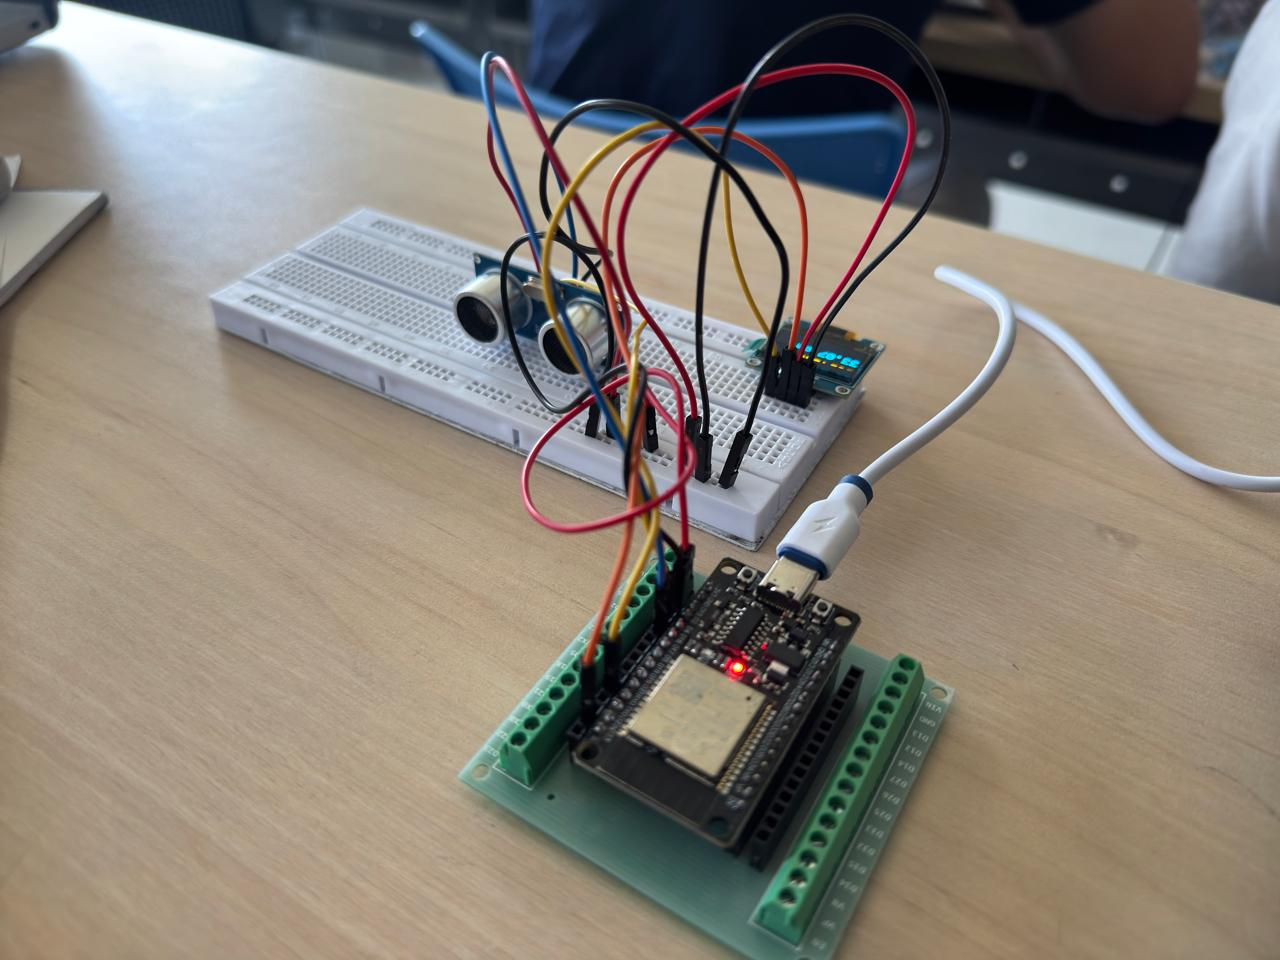
\includegraphics[width=\textwidth]{../Imagenes/Sensor_de_distacia_con_pantalla_imgs/Sensor_de_distancia_con_pantalla_img4.jpeg}
    \caption{Vista lateral del montaje completo: se observan claramente los dos transductores cilíndricos del HC-SR04 (emisor y receptor), la pantalla OLED con los datos y el ESP32 conectado por USB al computador.}
    \label{fig:img4}
\end{subfigure}
\caption{Montaje físico del sensor de distancia con pantalla OLED -- Detalles}
\label{fig:montaje2}
\end{figure}

% ══════════════════════════════════════════════════════════════
\section{Videos de Funcionamiento}
% ══════════════════════════════════════════════════════════════

Se dispone de tres videos que documentan el funcionamiento del proyecto:

\begin{itemize}
    \item \textbf{Sensor\_de\_distancia\_con\_pantalla\_Funcionamiento1.mp4}: Demostración principal del sistema midiendo distancias a diferentes objetos. Se observa cómo la pantalla OLED actualiza la lectura en tiempo real conforme se acercan y alejan objetos frente al sensor.
    \item \textbf{Sensor\_de\_distancia\_con\_pantalla\_Funcionamiento2.mp4}: Prueba del rango de medición del sensor, mostrando lecturas desde distancias cortas hasta el límite de detección del HC-SR04.
    \item \textbf{Sensor\_de\_distancia\_con\_pantalla\_Funcionamiento3.mp4}: Verificación de la lectura simultánea en la pantalla OLED y el monitor serial del Arduino IDE, confirmando que ambas interfaces muestran valores consistentes.
\end{itemize}

Estos videos se encuentran en la carpeta \texttt{Videos/Sensor\_de\_distancia\_con\_pantalla\_vid/} del repositorio del proyecto.

% ══════════════════════════════════════════════════════════════
\section{Proceso de Creación}
% ══════════════════════════════════════════════════════════════

El desarrollo del proyecto siguió un proceso incremental:

\begin{enumerate}
    \item \textbf{Montaje del sensor HC-SR04:} Se conectó el sensor a la protoboard con los pines Trig y Echo conectados a GPIO2 y GPIO4 del ESP32 respectivamente, alimentándolo con los pines de 3,3\,V y GND.
    
    \item \textbf{Prueba inicial por serial:} Se programó un sketch básico que solo leía el sensor y mostraba la distancia en el monitor serial, verificando que las lecturas fueran correctas y estables.
    
    \item \textbf{Conexión de la pantalla OLED:} Se conectó el display SSD1306 al bus I2C del ESP32 (SDA en GPIO21, SCL en GPIO22) con alimentación de 3,3\,V.
    
    \item \textbf{Instalación de librerías:} Se instalaron las librerías ``Adafruit SSD1306'' y ``Adafruit GFX Library'' desde el gestor de bibliotecas del Arduino IDE.
    
    \item \textbf{Integración del código:} Se combinó la lectura del sensor con la visualización en la pantalla OLED, configurando el tamaño de texto adecuado para que la lectura fuera legible en la pequeña pantalla de 0,96 pulgadas.
    
    \item \textbf{Ajuste y calibración:} Se verificó la precisión de las mediciones comparando con una regla, y se ajustó el delay entre lecturas a 500\,ms para un balance entre velocidad de actualización y estabilidad.
\end{enumerate}

% ══════════════════════════════════════════════════════════════
\section{Conceptos Técnicos Clave}
% ══════════════════════════════════════════════════════════════

\subsection{Velocidad del Sonido y Temperatura}

La velocidad del sonido en el aire depende de la temperatura según:
\begin{equation}
v_s = 331{,}3 + 0{,}606 \times T\,[\text{°C}] \quad [\text{m/s}]
\end{equation}

A 20\,°C: $v_s = 331{,}3 + 0{,}606 \times 20 = 343{,}4$\,m/s. El código utiliza un valor fijo (constante 58,4), lo que introduce un error menor del 1\% en el rango de 15--25\,°C.

\subsection{Función \texttt{pulseIn()}}

La función \texttt{pulseIn(pin, HIGH)} de Arduino mide la duración de un pulso digital. Internamente cuenta ciclos de reloj mientras el pin permanece en HIGH y devuelve el resultado en microsegundos. Tiene un timeout predeterminado de 1 segundo; si no detecta pulso, retorna 0.

\subsection{Búfer de la Pantalla OLED}

La librería Adafruit SSD1306 mantiene un búfer en RAM del ESP32 de 128$\times$64/8 = 1024 bytes, donde cada bit representa un píxel. Las funciones de dibujo modifican este búfer en memoria; solo al llamar \texttt{display.display()} se transfiere el búfer completo al controlador SSD1306 a través del bus I2C.

% ══════════════════════════════════════════════════════════════
\section{Conclusiones}
% ══════════════════════════════════════════════════════════════

\begin{itemize}
    \item El proyecto demuestra la integración exitosa de un sensor ultrasónico HC-SR04 con una pantalla OLED SSD1306 controlados por el ESP32, logrando un sistema de medición de distancia autónomo y portátil.
    \item La fórmula $d = t/58{,}4$ proporciona mediciones precisas dentro del rango operativo del sensor (2--400\,cm), basándose en la velocidad del sonido en el aire a temperatura ambiente.
    \item La comunicación I2C permite conectar la pantalla OLED con solo dos cables de datos (SDA y SCL), simplificando el cableado y dejando pines GPIO libres para otros periféricos.
    \item La visualización dual (monitor serial + pantalla OLED) permite tanto la depuración en el computador como el uso independiente del sistema, sin necesidad de mantener la conexión USB para ver las mediciones.
    \item Las librerías de Adafruit proporcionan una abstracción eficiente para el manejo gráfico de la pantalla OLED, facilitando la presentación de texto y valores numéricos con diferentes tamaños.
    \item El intervalo de actualización de 500\,ms ofrece un buen equilibrio entre velocidad de respuesta y estabilidad de las lecturas, evitando el parpadeo excesivo de la pantalla.
\end{itemize}

\end{document}
